\documentclass[10pt]{article}
\usepackage[web]{../problem-collection}
\newcommand{\pp}[1]{REMOVE}
\newcommand{\p}[1]{REMOVE}

\begin{document}

\begin{titlepage}
    \centering
    \vspace{10cm}
    {\sffamily\Huge \mbox{200 EESTI FÜÜSIKAOLÜMPIAADI}\\ ÜLESANNET AASTATEST\\ 2018 -- 2025\par}
    \vspace{1cm}
    {\Large koos vihjete ja lahendustega\par}
    \vfill
    {\Large Koostas Taavet Kalda}

    \vfill

    % Bottom of the page
    {\large 2025}
\end{titlepage}

\raggedbottom % Because of twosided
\mbox{}\vfill

\textcopyright~Autoriõigused: Eesti Matemaatika Selts, Tallinna Tehnikaülikool,
Tartu Ülikool, ülesannete autorid ja Taavet Kalda.
\vspace{0.5\baselineskip}

Kogumiku koostamist toetasid: Eesti Matemaatika Seltsi fond ``Benoit Mandelbroti Jälgedes'', Robert Kitt ja Tallinna Tehnikaülikool.
\vspace{0.5\baselineskip}

\newpage

\tableofcontents
\newpage

{\setlength{\parindent}{24pt}
\section{Sissejuhatus}

Siia on koondatud 200 gümnaasiumi ülesannet Eesti füüsikaolümpiaadi piirkonnavoorudest, lõppvoorudest ja lahtistest võistlustest. Igale ülesandele on juurde kirjutatud paarilauseline vihje. Juhul kui õpilane jääb ülesannet lahendades toppama, on tal võimalik vihjet lugeda ning teisele katsele minna.

%Tegu on teise kogumikuga Eesti füüsikaolümpiaadi ülesannete kogude seeriast, kus esimene kattis 200 ülesannet ajavahemikust 2012---2018.

Ülesanded on jaotatud teemade kaupa ning teemasiseselt raskuse järgi. Raskustaset tähistatakse kuni viie tärniga. Ülesannete lihtsamaks otsimiseks on ülesannete numbrite ette pandud \enquote{Ü}, vihjete ette \enquote{V} ja lahenduste ette \enquote{L}. Näiteks ülesande 133 teksti number on kujul Ü133. Iga ülesande juures on kirjas ka selle autor ning olümpiaadi vooru lühinimetus, lisaks lühendid P 1, G 1 jne, kus tähed tähistavad põhikooli- ja gümnaasiumiastet. Näiteks G 9 viitab gümnaasiumiastme 9. ülesandele.

%Kogumiku koostamise käigus eemaldati erinevatel põhjustel 3 ülesannet.

Lisaks leiate kogumiku lõpust kogumiku poolt kaetud lahtiste ja lõppvoorude esimese ja teise järgu saanud õpilaste ning ülesannete autorite nimekirja.}
\newpage
\setlength{\parindent}{0pt}

        \section{Ülesanded}
        \toggleStatement
        \subsection{\protect\StrSubstitute{Geomeetriline optika}{-}{ }}

\graphicspath{{../probs_b3/}}

% Ü1
\setAuthor{Erkki Tempel}
\setRound{lahtine}
\setYear{2018}
\setNumber{G 1}
\setDifficulty{1}
\setTopic{Geomeetriline optika}

\prob{Kärbes}
Kärbes asub kumerläätse fokaaltasandil, läätse optilisest peateljest kaugusel $a = \SI{1}{m}$ ning hakkab lendama läätse kahekordse fookuskauguse suunas kiirusega $v = \SI{0,5}{m/s}$. Läätse fookuskaugus $f = \SI{1}{m}$. Millise kiirusega $u$ liigub kärbse kujutis sel hetkel, kui kärbse ja tema kujutise vaheline kaugus on minimaalne?
\begin{center}
	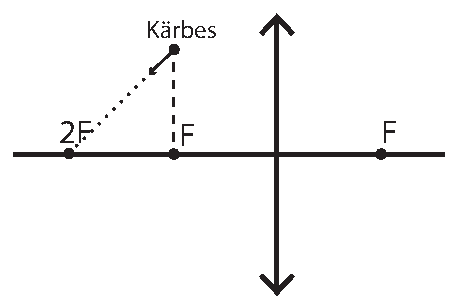
\includegraphics[width = 0.5\linewidth]{2018-lahg-01-yl.pdf}
\end{center}
\probend
\bigskip
\newpage\subsection{\protect\StrSubstitute{Elektriahelad}{-}{ }}

% Ü2
\setAuthor{Erkki Tempel}
\setRound{lahtine}
\setYear{2018}
\setNumber{G 2}
\setDifficulty{2}
\setTopic{Elektriahelad}

\prob{2018}
Sul on kasutada takistid $R_1=\SI{10}{\ohm}$, $R_2=\SI{100}{\ohm}$ ning $R_3=\SI{1000}{\ohm}$. Kasutades ainult neid takisteid, mooodustage kuuest takistist koosnev süsteem nii, et kogutakistus oleks $R=\SI{2018}{\ohm}\pm\SI{0,2}{\ohm}$.
\probend
\bigskip

% Ü3
\setAuthor{Jaan Kalda}
\setRound{lahtine}
\setYear{2018}
\setNumber{G 3}
\setDifficulty{3}
\setTopic{Elektriahelad}

\prob{Ring}
Traadist, mille ühe detsimeetri takistus on üks oom tehakse ring ümbermõõduga kuus detsimeetrit. Iga detsimeetri järel märgitakse punktid $a, b, \ldots, f$. Punktide $a$ ja $e$ vahele ühendatakse patarei pingega \SI{7}{V}, punktide $d$ ja $f$ vahele ampermeeter ning $d$ ja $b$ vahele voltmeeter. Punktid $f$ ja $b$ ühendatakse samast traadist lõigatud kahe-detsimeetrise traadijupiga. Leidke ampermeetri ja voltmeetri näidud.
\probend
\bigskip
\newpage\subsection{\protect\StrSubstitute{Dünaamika}{-}{ }}

% Ü4
\setAuthor{Erkki Tempel}
\setRound{lahtine}
\setYear{2018}
\setNumber{G 4}
\setDifficulty{4}
\setTopic{Dünaamika}

\prob{Kahurid}
Kahurist $A$ lastakse horisondi suhtes nurga $\alpha=\SI{30}{\degree}$ all lendu kuul algkiirusega $v_A=\SI{140}{m/s}$ kahuri $B$ suunas, mis on esimesest kahurist $l=\SI{1}{km}$ kaugusel samal tasapinnal. Sel hetkel, kui kuul on oma trajektoori kõrgeimas punktis, tulistatakse kahurist $B$ teine kuul, mis $t_1=\SI 5s$ pärast põrkub  esimese kuuliga. Millise algkiirusega tulistati kuul kahurist $B$? Õhutakistusega mitte arvestada; vabalangemise kiirendus $g\approx\SI{10}{m/s^2}$.
\probend
\bigskip
\newpage\subsection{\protect\StrSubstitute{Varia}{-}{ }}

% Ü5
\setAuthor{Andres Põldaru}
\setRound{lahtine}
\setYear{2018}
\setNumber{G 5}
\setDifficulty{5}
\setTopic{Varia}

\prob{Hiiglane}
Jukul vanem vend on tema kaks korda suuremaks skaleeritud identne koopia. Kas vanem vend hüppab kõrgemale kui Juku? Eeldage, et hüppeliigutus on mõlemal juhul täpselt sama ja et lihaste poolt tekitatav jõud sõltub ainult lihaste ristlõikepindalast. Hüppe kõrguse saamiseks lahutame pealae kõrgusest hüppaja pikkuse.
\probend
\bigskip
\newpage\subsection{\protect\StrSubstitute{Magnetism}{-}{ }}

% Ü6
\setAuthor{Kaarel Hänni}
\setRound{lahtine}
\setYear{2018}
\setNumber{G 6}
\setDifficulty{6}
\setTopic{Magnetism}

\prob{Magnetväljad}
Vaatleme prootoni liikumist x-y-tasandis. Vahemikus $0\leq x < \ell_1$ on magnetväli tugevusega $B$ $z$-telje positiivses suunas, vahemikus $\ell_1\leq x < \ell_1+\ell_2$ on magnetväli tugevusega $B$ $z$-telje negatiivses suunas. On teada, et $\ell_2 > \ell_1$. Ülejäänud tasandi osades magnetvälja pole. Alguses antakse prootonile mingi kiirus $\vec{v}$ tasandi vasakus pooles $x<0$. Milline on minimaalne kiirus $v=|\vec{v}|$, mille puhul saab valida sellise algse liikumissuuna, et prooton jõuab läbi kahe magnetväljaga vahemiku tasandi parempoolsesse osasse $x\geq \ell_1+\ell_2$? Prootoni laeng on $q$ ja mass on $m$.
\begin{center}
	\begin{tikzpicture}
	{
		\tikzset{ % This was originally used to update the global tikz style, but I prefer it to be locally defined instead
			odot/.style={
				circle,
				inner sep=0pt,
				node contents={$\odot$},
				scale=2
			},
			otimes/.style={
				circle,
				inner sep=0pt,
				node contents={$\otimes$},
				scale=2
			},
			circ/.style={
				circle,
				draw,
				minimum size=3mm,
				inner sep=0
			},
			odot2/.style={
				circ,
				path picture={\fill circle[radius=1pt];}
			},
			otimes2/.style={
				circ,
				path picture={
					\draw (path picture bounding box.45) -- (path picture bounding box.225);
					\draw (path picture bounding box.135) -- (path picture bounding box.315);
				}
			}
		}
		\draw[->] (-4,0) -- (4,0) node[below] {x};
		\draw[->] (-2,-2) -- (-2,3) node[left] {y};
		\draw (0,-2) -- (0,3);
		\draw (3,-2) -- (3,3);
		\draw[->] (-3.5,1) -- (-2.2,0.4) node[midway, below left] {$\vec{v}$};
		
		\draw [decorate,decoration={brace,amplitude=10pt}]
		(-2,0) -- (0,0) node [above, black,midway, yshift=7] {$\ell_1$}; 
		
		\draw [decorate,decoration={brace,amplitude=10pt}]
		(0,0) -- (3,0) node [above, black,midway, yshift=7] {$\ell_2$};
		
		\node [odot2] at (-1,2) {};
		\node [otimes2] at (1.5,2) {};
		\node at (-0.65,2) {$\vec{B}$};
		\node at (1.85,2) {$\vec{B}$};
	}
	\end{tikzpicture}
\end{center}
\probend
\bigskip

% Ü7
\setAuthor{Krister Kasemaa}
\setRound{lahtine}
\setYear{2018}
\setNumber{G 7}
\setDifficulty{7}
\setTopic{Dünaamika}

\prob{Kauss veega}
Kaalul olevasse kaussi hakatakse ühtlaselt pudelist kõrgusel $h$ vett valama. Vee valamine lõpetatakse hetkel, mil kaalu näit on $m$. Mis on kaalu lugem $M$ peale stabiliserumist? Kas see on esialgsest näidust suurem, väiksem või võrdne? Õhutakistusega mitte arvestada.
\probend
\bigskip
\newpage\subsection{\protect\StrSubstitute{Optika}{-}{ }}

% Ü8
\setAuthor{Jaan Kalda}
\setRound{lahtine}
\setYear{2018}
\setNumber{G 8}
\setDifficulty{8}
\setTopic{Optika}

\prob{Kolmnurk}
Joonisel on kujutatud täisnurkse kolmnurga kujutis (täisnurk on märgitud punktiga) õhukeses läätses, mis on koos oma peateljega samuti ära näidatud. Konstrueerida kolmnurga täisnurkse tipu tegelik asukoht.
\begin{center}
	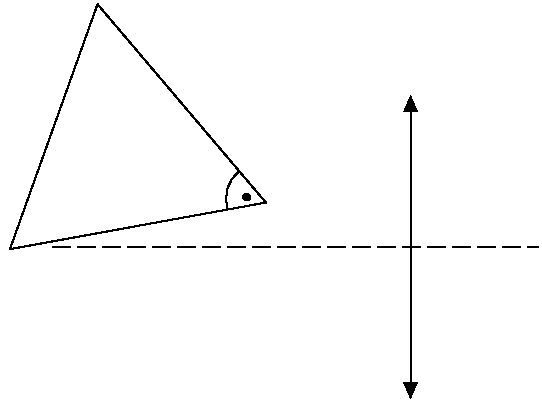
\includegraphics[width = 0.5\textwidth]{2018-lahg-08-yl.pdf}
\end{center}
\probend
\bigskip
\newpage\subsection{\protect\StrSubstitute{Termodünaamika}{-}{ }}

% Ü9
\setAuthor{Jaan Kalda}
\setRound{lahtine}
\setYear{2018}
\setNumber{G 9}
\setDifficulty{9}
\setTopic{Termodünaamika}

\prob{Õhkjahutus}
\begin{wrapfigure}[11]{r}{0.4\textwidth}
	\vspace{-20pt}
	\begin{center}
		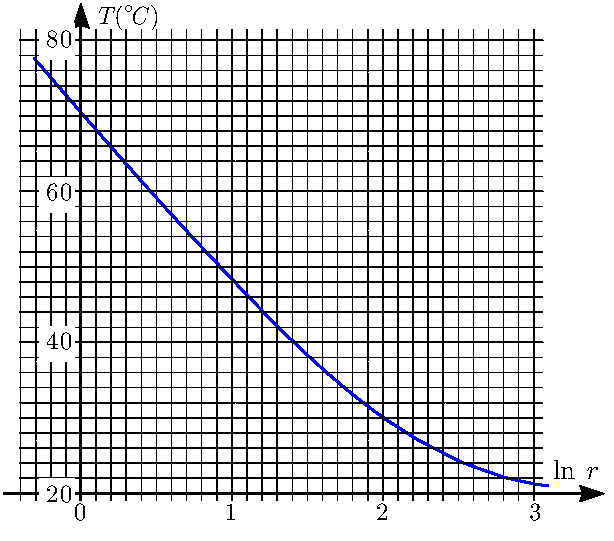
\includegraphics[width = \linewidth]{2018-lahg-09-yl.pdf}
	\end{center}
\end{wrapfigure}

\
Valgusdiood tarbib elektrilist võimsust $P=\SI{50}W$. Dioodi jahutamiseks on see kinnitatud vaskplaadile paksusega $t=\SI{500}{\micro m}$. Vase soojusjuhtivustegur $k=\SI{385}{W/m.K}$. Juuresoleval graafikul (suuremalt lisalehel) on toodud plaadi temperatuur sõltuvuses vaadeldava punkti ja dioodi vahelise kauguse naturaallogaritmist. Kauguse mõõtmiseks kasutatud ühikud ei ole teada. Dioodi mõõtmed lugeda tühiselt väikseks. Milline on dioodi kasutegur (milline osa tarvitatud elektrienergiast kiirgub valgusenergiana)?

\textit{Märkus:} soojusjuhtivustegur on arvuliselt võrdne soojusenergiaga, mis kandub materjalis läbi ühikulise ristlõikepindala, kui temperatuur langeb ühe kraadi võrra ühe pikkusühiku kohta.
\probend
\bigskip
\newpage\subsection{\protect\StrSubstitute{Kinemaatika}{-}{ }}

% Ü10
\setAuthor{Jaan Kalda}
\setRound{lahtine}
\setYear{2018}
\setNumber{G 10}
\setDifficulty{10}
\setTopic{Kinemaatika}

\prob{Pulk}
\begin{wrapfigure}[9]{r}{0.4\textwidth}
	\vspace{-15pt}
	\begin{center}
		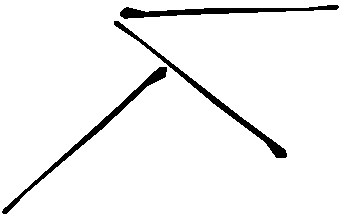
\includegraphics[width = 0.4\textwidth]{2018-lahg-10-yl.pdf}
	\end{center}
\end{wrapfigure}

Õhkuvisatud pulga lendu filmiti liikumatu videokaamera abil ja kahe võrdse intervalli tagant võetud kolm kaadrit kopeeriti juuresolevale joonisele (suuremalt lisalehel). On teada, et esimese ja viimase kasutatud kaadri vahele jäänud ajavahemiku jooksul jäi pulga pöördenurk väiksemaks täispöördest. Pulk pöörles joonise tasandis, pulga pikkus oli $L=\SI{1.0}m$ ja kaadri lühem külg on täpselt vertikaalne; raskuskiirendus $g=\SI{9.8}{m/s^2}$. Kui kaugel pulga jämedamast otsast asub selle massikese? Kui pikk oli esimese ja viimase kaadri vaheline ajavahemik?
\probend
\bigskip
\newpage\normalsize\section{Vihjed}
        \toggleHint
        
% V1
\setAuthor{Erkki Tempel}
\setRound{lahtine}
\setYear{2018}
\setNumber{G 1}
\setDifficulty{1}
\setTopic{Geomeetriline optika}

\prob{Kärbes}
\hint

\probend
\bigskip

% V2
\setAuthor{Erkki Tempel}
\setRound{lahtine}
\setYear{2018}
\setNumber{G 2}
\setDifficulty{2}
\setTopic{Elektriahelad}

\prob{2018}
\hint

\probend
\bigskip

% V3
\setAuthor{Jaan Kalda}
\setRound{lahtine}
\setYear{2018}
\setNumber{G 3}
\setDifficulty{3}
\setTopic{Elektriahelad}

\prob{Ring}
\hint

\probend
\bigskip

% V4
\setAuthor{Erkki Tempel}
\setRound{lahtine}
\setYear{2018}
\setNumber{G 4}
\setDifficulty{4}
\setTopic{Dünaamika}

\prob{Kahurid}
\hint

\probend
\bigskip

% V5
\setAuthor{Andres Põldaru}
\setRound{lahtine}
\setYear{2018}
\setNumber{G 5}
\setDifficulty{5}
\setTopic{Varia}

\prob{Hiiglane}
\hint

\probend
\bigskip

% V6
\setAuthor{Kaarel Hänni}
\setRound{lahtine}
\setYear{2018}
\setNumber{G 6}
\setDifficulty{6}
\setTopic{Magnetism}

\prob{Magnetväljad}
\hint

\probend
\bigskip

% V7
\setAuthor{Krister Kasemaa}
\setRound{lahtine}
\setYear{2018}
\setNumber{G 7}
\setDifficulty{7}
\setTopic{Dünaamika}

\prob{Kauss veega}
\hint

\probend
\bigskip

% V8
\setAuthor{Jaan Kalda}
\setRound{lahtine}
\setYear{2018}
\setNumber{G 8}
\setDifficulty{8}
\setTopic{Optika}

\prob{Kolmnurk}
\hint

\probend
\bigskip

% V9
\setAuthor{Jaan Kalda}
\setRound{lahtine}
\setYear{2018}
\setNumber{G 9}
\setDifficulty{9}
\setTopic{Termodünaamika}

\prob{Õhkjahutus}
\hint

\probend
\bigskip

% V10
\setAuthor{Jaan Kalda}
\setRound{lahtine}
\setYear{2018}
\setNumber{G 10}
\setDifficulty{10}
\setTopic{Kinemaatika}

\prob{Pulk}
\hint

\probend
\bigskip
\newpage\section{Lahendused}
        \toggleSolution
        
% L1
\setAuthor{Erkki Tempel}
\setRound{lahtine}
\setYear{2018}
\setNumber{G 1}
\setDifficulty{1}
\setTopic{Geomeetriline optika}

\prob{Kärbes}
\solu
Minimaalne kaugus on siis, kui kärbes läbib optilist peatelge. Kärbes ja tema kujutis on sel hetkel läätsest kahekordse fookuskauguse kaugusel. Kuna nii kärbes kui ka tema kujutis on läätsest sama kaugel, on kujutise suurendus $1$, mistõttu kujutise liikumiskiirus on sama, mis kärbse liikumiskiirus, ehk $u = v = \SI{0,5}{m/s}$.
\probend
\bigskip

% L2
\setAuthor{Erkki Tempel}
\setRound{lahtine}
\setYear{2018}
\setNumber{G 2}
\setDifficulty{2}
\setTopic{Elektriahelad}

\prob{2018}
\solu
Selleks, et kogutakistus oleks $\SI{2018}{\ohm}$, peaks kaks $R_3$ takistit ülejäänud takistitega jadamisi olema. Pannes need rööbiti muutuks takistus liiga väikseks. Seega taandub ülesanne $\SI{18}{\ohm}\pm\SI{0.2}{\ohm}$ leidmisele nelja takistiga. Üks sobilikest lahenditest on näiteks kahe $R_1$ ja kahe $R_2$ rööbiti paigutamine. Sellisel juhul on takistus $2R_3 + \frac{1}{\frac{1}{2R_1} + \frac{1}{2R_2}} = \SI{2018.182}{\ohm}$
\probend
\bigskip

% L3
\setAuthor{Jaan Kalda}
\setRound{lahtine}
\setYear{2018}
\setNumber{G 3}
\setDifficulty{3}
\setTopic{Elektriahelad}

\prob{Ring}
\solu
\begin{wrapfigure}[11]{r}{0.4\textwidth}
	\vspace{-20pt}
	\begin{center}
		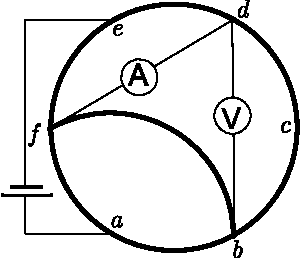
\includegraphics[width = 0.4\textwidth]{2018-lahg-03-yl.pdf}
	\end{center}
\end{wrapfigure}

Teeme ekvivalentskeemi, vt joonis, kus ideaalse ampermeetri asendame traadiga ning ideaalse voltmeetri kõrvaldame. Et voltmeeter on kinnitatud punktide $b$ ja $d$ vahele, siis peame leidma pinge takistil $2R$. Kirhoffi vooluseaduse tõttu näitab ampermeeter ülemise vasakpoolse takisti $R$ ning ülemise takisti $2R$ voolude vahet. Takistus $d$ ja $a$ vahel on takistite $R$ ja $2R$ rööpühendus, st $\frac 23R$ ning $d$ ja $e$ vahel --- $\frac 12R$; seega kogutakistus on $\frac 76R$. Voolutugevus läbi patarei on $I_0=\frac 67\frac{\mathcal E}R$ ning see jaguneb punkte $d$ ja $a$ ühendava ülemise ja alumise haru vahel takistuste suhte vahekorras 1:2, st ülemisse harru läheb vool $I=\frac 13I_0=\frac 27\frac{\mathcal E}R$. Pinge $d$ ja $b$ vahel saame Ohmi seadusest, $U=IR=\frac 27\mathcal E=\SI 2V$. Läbi ülemise vasakpoolse takisti läheb pool koguvoolust, $I_1=\frac 12 I_0=\frac 37\mathcal E$ ja takistit $2R$ läbib vool $I_2=\frac U{2R}= \frac 17\mathcal E$. Seega ampermeeter näitab voolu $I_A=I_2-I_1=\frac{2\mathcal E}{7R}=\SI 2A$.
\probend
\bigskip

% L4
\setAuthor{Erkki Tempel}
\setRound{lahtine}
\setYear{2018}
\setNumber{G 4}
\setDifficulty{4}
\setTopic{Dünaamika}

\prob{Kahurid}
\solu
\
Kahurist $A$ tulistatud kuul jõuab haripunkti siis, kui selle vertikaalne kiiruse komponent on $0$, ehk ajahetkel $t_0 = \frac{v_A\sin\alpha}{g} = \SI{7}{s}$. Kahurikuulid põrkuvad seega kokku momendil $t_0 + t_1 = \SI{12}s$. Sellel hetkel on kahurist $A$ lastud kuuli ja kahuri $B$ horisontaalne vahekaugus $v_A\cos\alpha(t_0 + t_1) - l = v_{Bx}t_1$, kus $v_B$ on kahurist $B$ tulistatud kuuli algkiirus. Niisiis, $v_{Bx} = \frac{v_A\cos\alpha(t_0 + t_1) - l}{t_1} = \SI{-91.0}{m/s}$.

Selleks, et kuulid vertikaaltasandis ajehetkel $t_0 + t_1$ kokku saaksid, peab kehtima
\[
v_A\sin\alpha (t_0 + t_1) - \frac{g(t_0 + t_1)^2}{2} = v_yt - \frac{gt_1^2}{2},
\]
ehk
\[
v_{B_y} = v_A\sin\alpha \left(\frac{t_0}{t_1} + 1\right) - \frac{g(t_0 + t_1)^2}{2t_1} + \frac{gt_1}{2} = \SI{49}{m/s}.
\]
Niisiis,
\[
v_B = \sqrt{v_{Bx}^2 + v_{By}^2} = \SI{103}{m/s}.
\]
\probend
\bigskip

% L5
\setAuthor{Andres Põldaru}
\setRound{lahtine}
\setYear{2018}
\setNumber{G 5}
\setDifficulty{5}
\setTopic{Varia}

\prob{Hiiglane}
\solu
Võrdleme mõlema hüppaja poolt tehtud tööd. Läbides väikese vahemaa $\Delta l$ teevad lihased töö
$$\Delta A = F \Delta l.$$
Jõud sõltub hüppaja kõrgusest $h$ ruutsõltuvuse järgi, sest lihaste pindala kasvab lineaarmõõtme ruuduga. Lisaks kasvab läbitud vahemaa võrdeliselt lineaarmõõtmega. Seega lihaste poolt tehtud töö on võrdeline hüppaja pikkuse kuubiga $A \propto h^3$.

Vaatleme nüüd, kui palju potentsiaalne energia muutub. Algselt seisab hüppaja vabalt, seejärel laskub alla vahemaa $h_1$ võrra ja hüppab üles. Kui hüppe kõrgus on $h_2$, siis potentsiaalsete energiate vahemaa hüppe madalaimas ja kõrgeimas punktis on $mg(h_1+h_2)$. Kuna alg- ja lõpphetkel on hüppaja paigal (kineetiline energia puudub), siis energia jäävuse seaduse järgi peab tehtud töö võrduma potentsiaalse energia muuduga:
$$A = mg(h_1+h_2) \quad\rightarrow\quad h_2 = \frac{A}{mg} - h_1.$$
Kuna nii mass kui tehtud töö $A$ sõltuvad lineaarmõõtme kuubist, siis jagatis $A/m$ on mõlema hüppaja jaoks sama. Kuna laskumise vahemaa $h_1$ on võrdeline hüppaja pikkusega, siis tuleb välja, et hüppe kõrgus on suuremal vennal hoopis väiksem.
\probend
\bigskip

% L6
\setAuthor{Kaarel Hänni}
\setRound{lahtine}
\setYear{2018}
\setNumber{G 6}
\setDifficulty{6}
\setTopic{Magnetism}

\prob{Magnetväljad}
\solu
Magnetväljas tugevusega $B$ liigub prooton kiirusega $v$ ringjoonelisel trajektooril raadiusega $R$. Tsentripetaaljõu ja magnetjõu võrdusest saab avaldada $R$:
\[\frac{mv^2}{R}=qvB\implies R=\frac{mv}{qB}.\]
Prootoni trajektoor vahemikus $\ell_1\leq x < \ell_1+\ell_2$ on ringjoon (täpsemalt ringjoone kaar), mis lõikub sirgega $x=\ell_1$. Et prooton saaks jõuda tasandi parempoolsesse osasse $x\geq \ell_1+\ell_2$, peab selle trajektoor lõikuma ka sirgega $x=\ell_1+\ell_2$. Seega peab selle trajektoorile vastav ringjoon lõikuma kahe paralleelse sirgega, mille vahekaugus on $\ell_2$. Siit $2R \geq \ell_2$ ehk $2\frac{mv}{qB}\geq \ell_2$, millest $v\geq \frac{qB\ell_2}{2m}$. Kui prooton siseneb teise vahemikku liikudes vertikaalsihis alla kiirusega $v= \frac{qB\ell_2}{2m}$, siis selle trajektoor on poolkaar, millel liikudes see jõuab täpselt vahemikust läbi. Kuna $\ell_1<\ell_2$, siis leidub selline prootoni sisenemisnurk esimesse vahemikku, mille puhul prooton jõuab teise vahemikku. Kui keerata sellest sisenemisnurgast alustades prootoni kiirusvektorit päripäeva, siis vertikaalse vektorini jõudes selle trajektoor enam sirget $x=\ell_1$ ei lõika. Seega mingil hetkel puutub selle trajektoorile vastav ringjoon sirget $x=\ell_1$. Selle sisenemisnurga puhul läbib prooton esimese vahemiku ja siseneb teise vahemikku vertikaalselt alla mineva kiirusega, seega see läbib mõlemad vahemikud. Seega on kiiruse $v=\frac{qB\ell_2}{2m}$ puhul prootonil võimalik tasandi vasakpoolsest osast tasandi parempoolsesse osadesse saada. Näitasime juba, et väiksemad kiirused ei tööta, seega minimaalne läbimiskiirus on $v=\frac{qB\ell_2}{2m}$.

\begin{centering}
	{
		\tikzset{
			odot/.style={
				circle,
				inner sep=0pt,
				node contents={$\odot$},
				scale=2
			},
			otimes/.style={
				circle,
				inner sep=0pt,
				node contents={$\otimes$},
				scale=2
			},
			circ/.style={
				circle,
				draw,
				minimum size=3mm,
				inner sep=0
			},
			odot2/.style={
				circ,
				path picture={\fill circle[radius=1pt];}
			},
			otimes2/.style={
				circ,
				path picture={
					\draw (path picture bounding box.45) -- (path picture bounding box.225);
					\draw (path picture bounding box.135) -- (path picture bounding box.315);
				}
			}
		}
		\begin{tikzpicture}
		1.40953893117
		0.48969832121
		1.34543507989
		\draw[->] (-4,0) -- (4,0) node[below] {x};
		\draw[->] (-2,-2) -- (-2,3) node[left] {y};
		\draw (0,-2) -- (0,3);
		\draw (3,-2) -- (3,3);
		\draw[->] (-3.34543507989,0.91984060996) -- (-2,1.40953893117) node[midway, below left] {$\vec{v}$};
		
		\draw [decorate,decoration={brace,amplitude=10pt}]
		(-2,0) -- (0,0) node [above, black,midway, yshift=7] {$\ell_1$}; 
		
		\draw [decorate,decoration={brace,amplitude=10pt}]
		(0,0) -- (3,0) node [above, black,midway, yshift=7] {$\ell_2$};
		
		\node [odot2] at (-1,2) {};
		\node [otimes2] at (1.5,2) {};
		\node at (-0.65,2) {$\vec{B}$};
		\node at (1.85,2) {$\vec{B}$};
		
		\draw [thick, dotted,domain=180:360] plot ({1.5+1.5*cos(\x)}, {1.5*sin(\x)});
		\draw [thick, dotted,domain=110:0] plot ({-1.5+1.5*cos(\x)}, {1.5*sin(\x)});
		
		
		\end{tikzpicture}
	}
	
\end{centering}
\probend
\bigskip

% L7
\setAuthor{Krister Kasemaa}
\setRound{lahtine}
\setYear{2018}
\setNumber{G 7}
\setDifficulty{7}
\setTopic{Dünaamika}

\prob{Kauss veega}
\solu
Käsitleme esmalt jõudu mida põhjustab veesamba impulsi muut kausile, jättes kõrvale veesamba massi mis langeb kaussi peale valamise lõppemist. Veesammas mõjub kausi põhjale jõuga $F=\frac{dp}{dt}$. Olgu vee kiirus vahetult enne põhja vastu põrkumist $v$. Võime teha lihtsustuse, et kausi põhja vastu põrkudes jääb vesi seisma. Seega,
\[
F=\frac{\mathrm{d}{p}}{\mathrm{d}{t}}=\frac{\mathrm{d}{m}}{\mathrm{d}{t}} |v|.
\]\par 
\noindent Järgmiseks leiame vee kiiruse vahetult enne kaussi jõudmist.  Valamise algushetkel on vee kiirus $v_0\approx 0$. Langedes rakendab veesambale jõudu ainult gravitatsioon. Seega rakendame valemit $v^2-v_0^2=2a\Delta s$, millest avaldub, et $v=\sqrt{2hg}$
Järelikult $F=\frac{\mathrm{d}{m}}{\mathrm{d}{t}} |v|=\frac{\mathrm{d}{m}}{\mathrm{d}{t}}\sqrt{2gh}$
Vee valamine lõpetati hetkel, kui $m_{\mathrm{kausis}} g+F=m_\mathrm{skaalal}g$, millest avaldub, et vee mass valamise hetkel kausis oli:
\begin{equation*}
m_{\mathrm{kausis}}=\frac{m_{\mathrm{skaalal}} g-F}{g}=m_{\mathrm{skaalal}}-\frac{\mathrm{d}{m}}{\mathrm{d}{t}}\sqrt{\frac{2h}{g}}.
\end{equation*}
Käsitleme nüüd veesamba massi, mis lisandub kaussi peale valamise lõppemist. Veesamba mass on $m_{\mathrm{veesammas}}=\frac{\mathrm{d}{m}}{\mathrm{d}{t}}\Delta t$, kus $\Delta t$ on aeg mil kulub veesamba ühe elementaarelemendi jõudmiseks kaussi. Rakendame valemit$v=v_0+at$ ja leiame, et:
\begin{equation*}
\Delta t = \frac{v-v_0}{g}=\frac{v}{g}=\sqrt{\frac{2h}{g}}.
\end{equation*}
Millest järeldub, et valamise lõppedes on kaussi jõudva veesamba mass on
\begin{equation*}
m_{\mathrm{veesammas}}=\frac{\mathrm{d}{m}}{\mathrm{d}{t}} \Delta t = \frac{\mathrm{d}{m}}{\mathrm{d}{t}}\sqrt{\frac{2h}{g}}.
\end{equation*}
Nüüd saame leida vee massi $M$, mis jõuab kaussi:
\begin{equation*}
M=m_{\mathrm{kausis}}+m_{\mathrm{veesammas}}=m_{\mathrm{skaalal}}-\frac{\mathrm{d}{m}}{\mathrm{d}{t}}\sqrt{\frac{2h}{g}}+\frac{\mathrm{d}{m}}{\mathrm{d}{t}}\sqrt{\frac{2h}{g}}=m_{\mathrm{skaalal}}.
\end{equation*}
\probend
\bigskip

% L8
\setAuthor{Jaan Kalda}
\setRound{lahtine}
\setYear{2018}
\setNumber{G 8}
\setDifficulty{8}
\setTopic{Optika}

\prob{Kolmnurk}
\solu
Tähistame kolmnurga kujutise tähtedega $ABC$ (vt joonis) ja olgu täisnurkse tipu kujutisele $C$ vastav originaal punktis $F$. Paneme tähele, et sirge kujutis on sirge ning need kaks sirget lõikuvad läätse tasandis. Lõikugu küljega $AC$ määratud sirge läätse tasandiga punktis $D$ ning olgu selle sirge kujutis sirge $DF$. Analoogselt defineerime sirge 
$BC$ abil punkti $E$ ja sirge $FE$. Et $\angle DFE$ on ülesande tingimuse kohaselt täisnurk, siis peab see asuma ringjoonel, mis on ehitatud lõigule $DE$ kui diameetrile.Teisest küljest punktist $C$ läbi läätse keskpunkti tõmmatud kiir läätses ei murdu ja seetõttu peab punkt $F$ asuma sellel kiirel. Niisiis leiamegi otsitava punkti $F$ kui antud kiire ja ringjoone lõikepunkti.
\begin{center}
	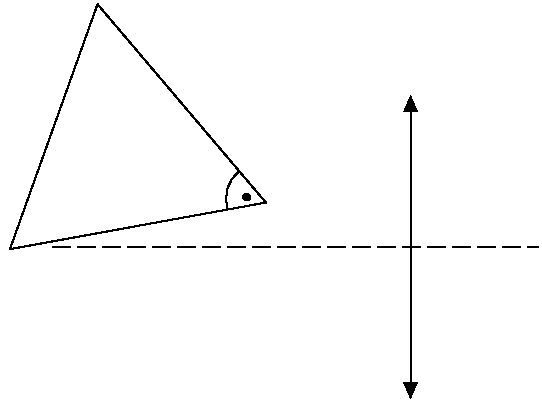
\includegraphics[width=0.5\linewidth]{2018-lahg-08-yl.pdf}
\end{center}
\probend
\bigskip

% L9
\setAuthor{Jaan Kalda}
\setRound{lahtine}
\setYear{2018}
\setNumber{G 9}
\setDifficulty{9}
\setTopic{Termodünaamika}

\prob{Õhkjahutus}
\solu
\
Piirkonnas, mis on dioodile lähedal ja kus seetõttu mööda plaati leviv soojusenergia pole veel jõudnud õhku kaduda, on soojusvoog $P_s=2\pi rtk \frac{\mathrm d T}{\mathrm d r}=2\pi tk \frac{\mathrm d T}{\mathrm d \ln r}$, kus $P_s$ on soojusena dissipeeruv soojusvõimsus. Näeme, et selles piirkonnas, kus antud eeldus kehtib, peab graafik olema sirgjoon ja selle tõus võrduma $\tan\alpha=2\pi tk$. Graafikul on väikeste $r$ väärtuste juures tõepoolest selline piirkond olemas ning graafiku puutuja tõus on seal $\tan\alpha\approx\SI{23.5}K$. Seega $P_s=kt\cdot \SI{23.5}K\approx \SI{28.5}W$. Kiiratud võimsus $P_k=P-P_s$ ning kasutegur $\eta=P_s/P\approx 0.43$.
\probend
\bigskip

% L10
\setAuthor{Jaan Kalda}
\setRound{lahtine}
\setYear{2018}
\setNumber{G 10}
\setDifficulty{10}
\setTopic{Kinemaatika}

\prob{Pulk}
\solu
Esimese ja teise kaadri-intervalli jooksul pöördus pulk sama nurga võrra, see tähendab, et peaaegu horisontaalne pulga asend peab pärinema keskmiselt kaadrilt ja ülejäänud asendid on ca $\pm 140^\circ$ võrra pööratud. Üldsust kitsendamata võime eeldada, et vasak alumine asend vastab esimesele kaadrile (kui see vastab tegelikult viimasele, siis vaatleme pulga liikumist tagurpidi kulgevas ajas). Jooniselt teeme kindlaks, et esimese kaadriintervalli jooksul nihkus pulga peenem ots horisontaalsihis paremale ca $p_1=\SI{155}{cm}$ võrra ja jämedam ots --- $j_1=\SI{-20}{cm}$  võrra. Et teatud pulga punkti horisontaalne nihe esimese kaadriintervalli jooksul $s_1$ on lineaarne funktsioon selle punkti kaugusest $x$ pulga jämedamast otspunktist, siis $s_1=p_1\frac xL+j_1(1-\frac xL)$, kus $L$ tähistab pulga pikkust. Analoogselt leiame nihked teise kaadriintervalli jaoks $p_2=\SI{-105}{cm}$ ja $j_2=\SI{75}{cm}$ ning $s_2=p_2\frac xL+j_2(1-\frac xL)$. Et massikeskme horisontaalne kiiruskomponent ei muutu, siis $s_1=s_2$, millest $\frac xL(p_1-p_2+j_2-j_1)=j_2-j_1$, st $x=L\frac{95}{355}\approx \SI{27}{cm}$.

Teeme nüüd jooniselt kindlaks massikeskme vertikaalsihilised nihked: $v_1=\SI{45}{cm}$ ja $v_2=\SI{-50}{cm}$.
Olgu kaadriintervall $\tau$; massikeskme keskmine kiirus esimese kaadriintervalli jooksul oli $v_1/\tau$ ja teise jooksul --- $v_2/\tau$ ning muutus - $(v_2-v_1)/\tau= -g\tau$, seega $\tau=\sqrt{(v_1-v_2)/g}\approx \SI{0.31}s$.
\probend
\bigskip
\newpage

\section{Autorite loetelu}

TODO

\end{document}